\begin{figure*}
\centering
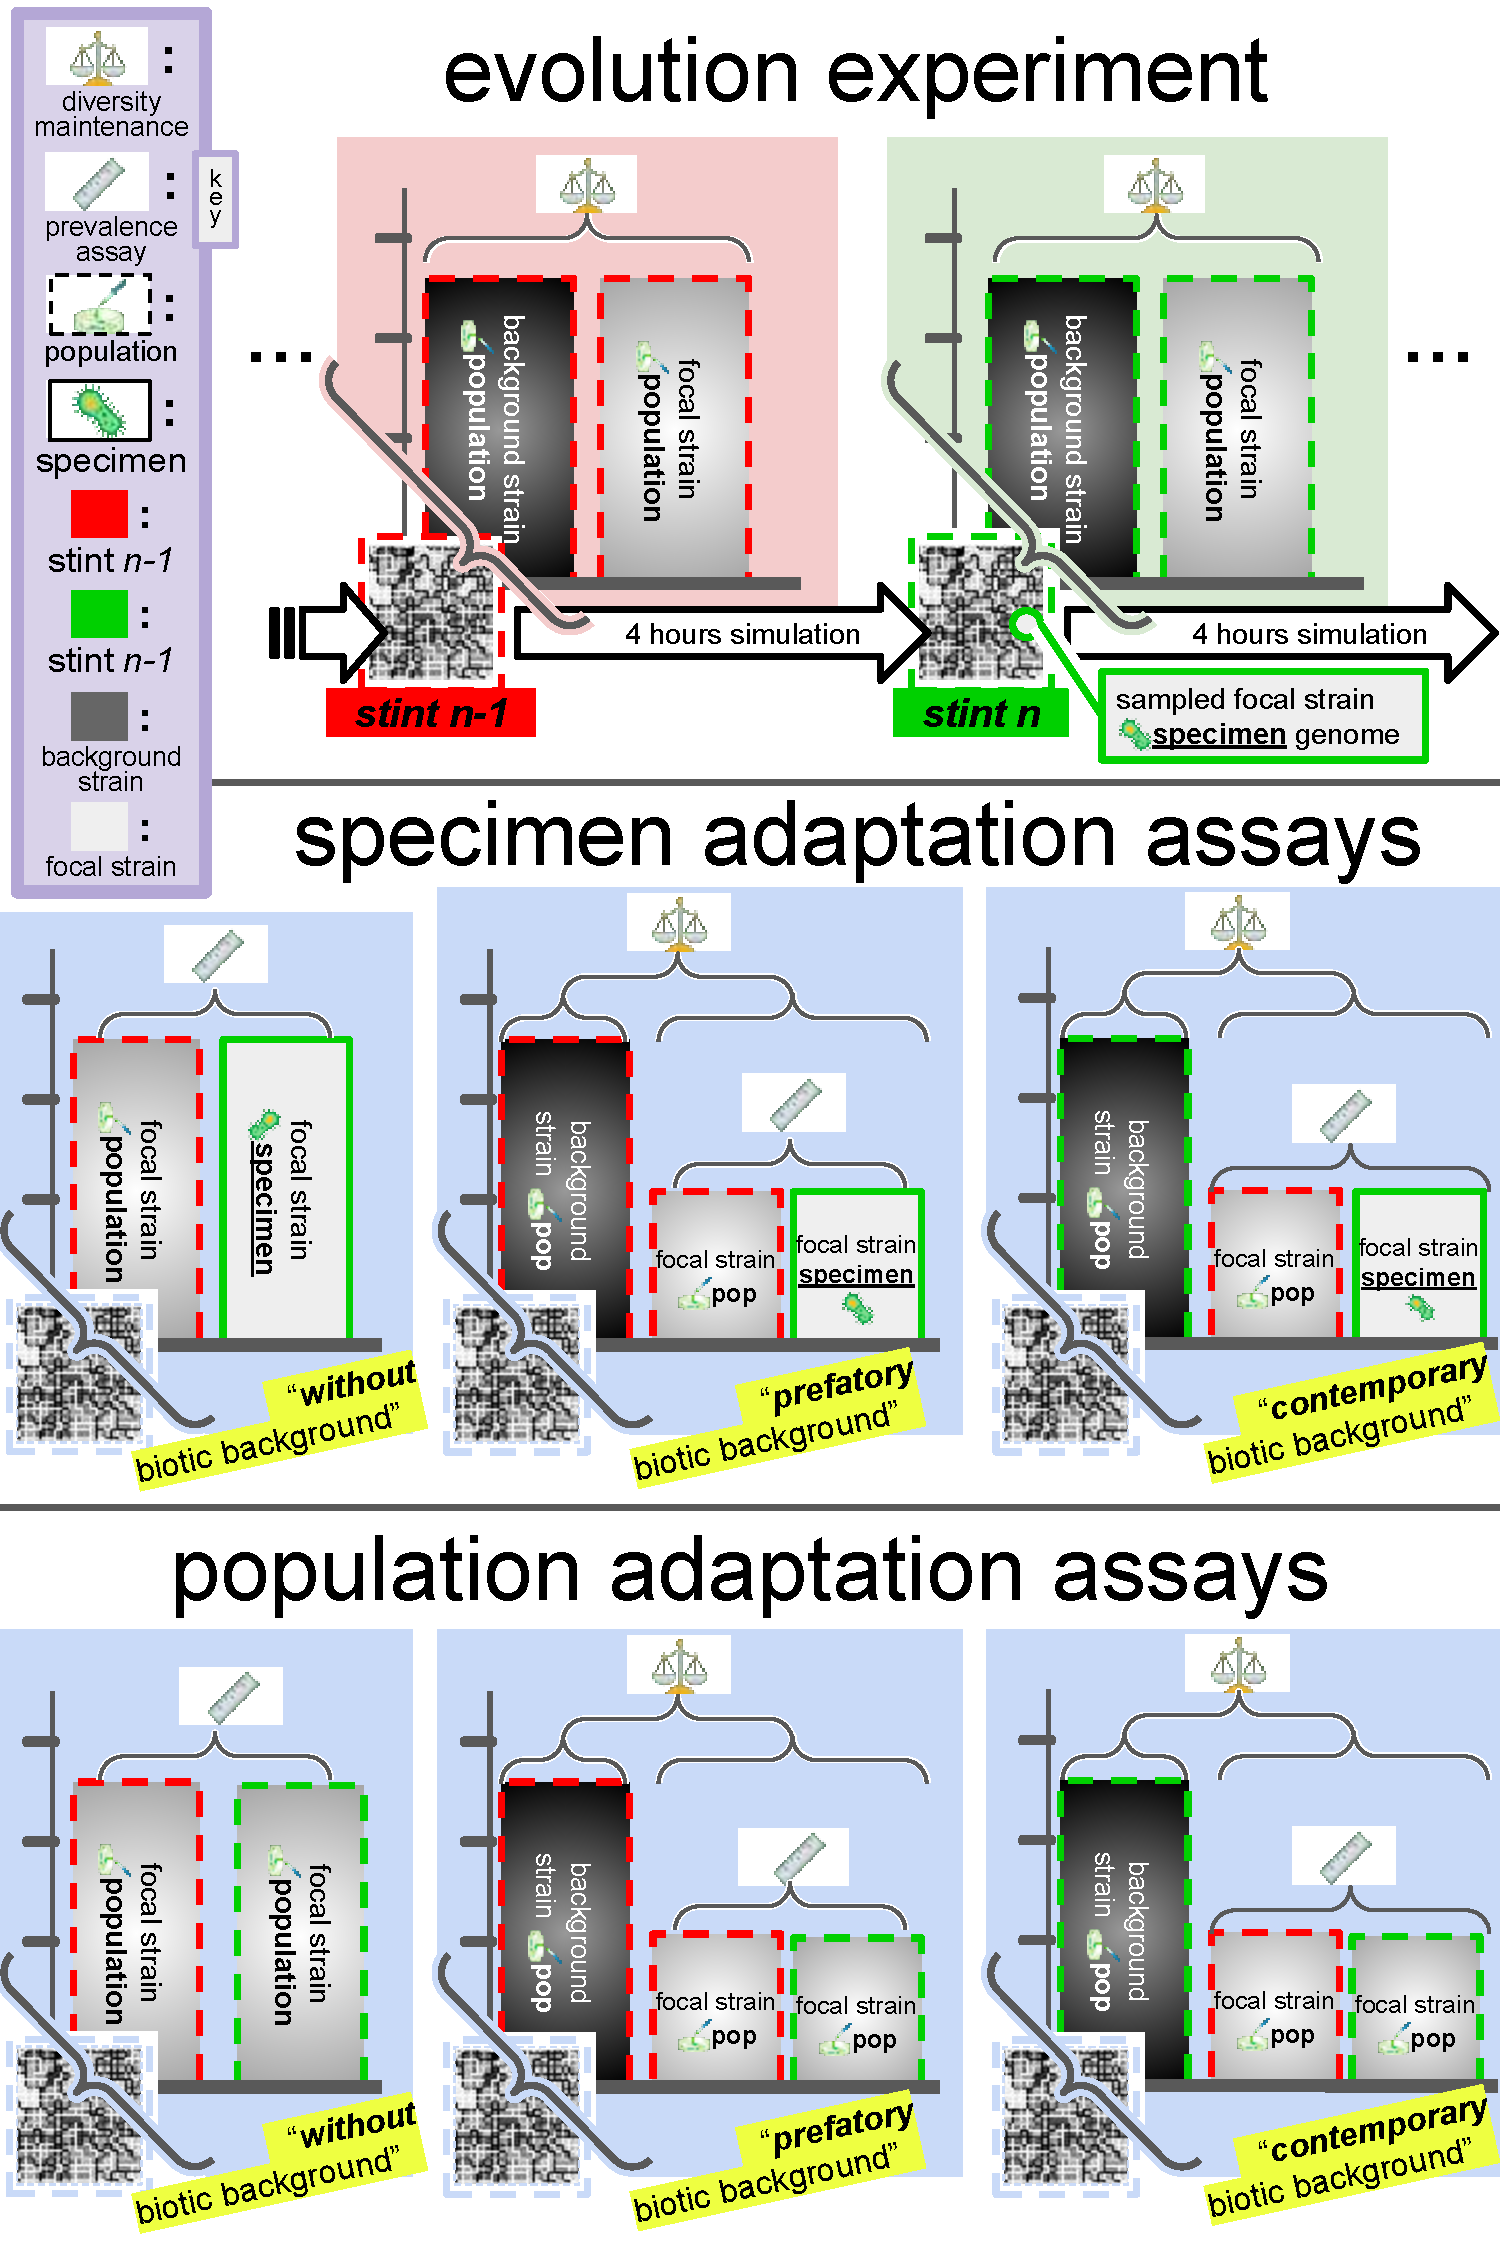
\includegraphics[width=0.5\linewidth]{{img/adaptation-assay-cartoon}}

\caption{
\textbf{Adaptation assay design.}
\footnotesize
Top panel shows progress of original evolutionary experiment over one stint.
A diversity maintenance procedure was used to ensure long-term coexistence of at least two strains over the course of the experiment by penalizing any strain that occupied more than half of thread-local population space.
A ``focal strain'' was arbitrarily chosen for study; we refer to the other strain as the ``background strain.''
Adaptation assays in lower panels measure fitness change over the course of that stint through competition against the population from the preceding stint.
The middle panel shows measurement of adaptation of the representative specimen that was sampled for analysis at each stint.
The bottom panel shows measurement of the adaptation of the entire focal strain population at each stint.
Competitors were mixed in even proportion into the environment.
Bar heights represent initial relative proportions of assay participants at the beginning of the competition.
Adaptation was measured by measuring change in population composition over a 10 minute competition window.
We call this measurement of population composition change a ``prevalence assay''.
Competition experiments were performed absent the background strain, with the background strain population from the preceding stint, or with the background strain population from the current stint --- shown separately in each panel.
}
\label{fig:adaptation_assay_cartoon}
\end{figure*}
